\section{Механизмы конкурентного внимания\\{и ограничения разделения-восстановления}}
\begin{center}
\emph{Механизмы конкурентного внимания}\\
\emph{и ограничения разделения-восстановления}
\end{center}
\par Часть разделения стиля темы пред- назначена для создания распределенных 
представлений темы и стиля соответствен- но. Стилевое представление используется 
для основной задачи: установления авторства, а тематическое – для вспомогательной 
задачи: аппроксимации темы.

\begin{figure}[!ht]
    \begin{center}
    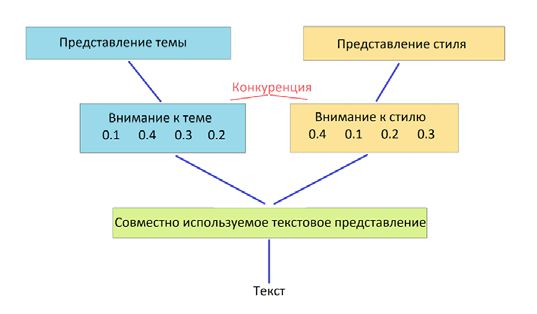
\includegraphics[scale=1.0]{images/pic1.jpg}
    \caption{Механизм конкурентного внимания}
    \label{fig:pic21}
    \end{center}
\end{figure}

\begin{figure}[!ht]
    \begin{center}
    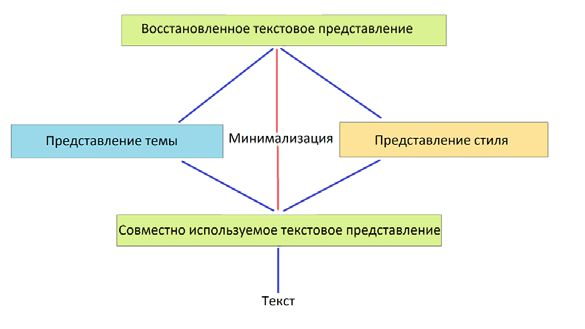
\includegraphics[scale=1.0]{images/pic2.jpg}
    \caption{Ограничение разделения-восстановления}
    \label{fig:pic2}
    \end{center}
\end{figure}

\par Для достижения поставленных целей 
предлагаются две идеи: механизм конкурентного внимания и ограничение разделения-восстановления. Рисунки 1 и 2 иллюстрируют две идеи. 
\par Конкурентное внимание – это расширение механизма внимания, который учится присваивать разные веса разным токенам. 
Здесь мы используем внимание, чтобы выделить общее текстовое представление, чтобы получить отдельные представления для темы и стиля. 
Если слову уделяется большое внимание для одной задачи, ему будет отведено низкое внимание для другой задачи. 
Другими словами, два представления конкурируют за внимание каждого слова.
\par Ограничение разделения-восстановления вводит затраты на восстановление в дополнение к оптимизации двух вышеупомянутых задач. Ожидается, что представления 
темы и стиля могут реконструировать представление текста, чтобы сохранить исходное значение.

\section{Конкурентное внимание для разделения темы и стиля}
\begin{center}
\emph{Конкурентное внимание}\\
\emph{для разделения темы и стиля}
\end{center}
\par Рекуррентная нейронная сеть (RNN) 
подходит для обработки последовательных 
данных и для захвата долгосрочных зависимостей. RNN используется в качестве базовой архитектуры в этой работе [2].
\begin{enumerate}[label={\arabic*)}, left=10pt]
\item LSTM на основе внимания
\paragraph*{} Слова текста преобразуются во вложения слов, которые представляют собой 
плотные векторы действительных значений. Входной текст может быть представлен в виде матриц
\[
\mathit{W} = (w_1, \ldots, w_n) \in \mathds{\mathrm{R}}^{d \times r}
\]
где $d$ – размер встраивания, а $n$ – количество токенов в тексте. В качестве основной 
ячейки памяти мы используем долговременную кратковременную память (LSTM). 
На временном шаге $t$ LSTM берет скрытое 
состояние с предыдущего временного шага 
и встраивание слова с текущего шага в качестве входных данных и создает новое скрытое состояние [3].
\begin{equation}
    \textit{h}_t = \textit{LSTM}(w_t, h_{t-1})
\end{equation}
\paragraph*{} Вся последовательность создает $n$ скрытых состояний, представленных как $\mathit{H} = (h_1, \ldots, h_t)$ . Сначала мы получаем $u_i$, скрытое представление $h_i$, через многослойный персептрон (\textit{MLP}).
\begin{equation}
    \textit{u}_i = tanh (Mh_i+b)
\end{equation}
\paragraph*{}Затем вводится контекстный вектор $u_c$
для вычисления весов токенов.
\begin{equation}
    \alpha_i = \frac{exp(u^T_iu_c)}{\sum_i(u^T_iu_c)}
\end{equation}
где $u_c$ является общим для всех текстов 
и случайным образом инициируется и обновляется во время обучения.
\paragraph*{} При векторе внимания окончательное представление текста является взвешенной суммой скрытых состояний [4],
\begin{equation}
    h^{*} = \sum^n_i{\alpha_i h_i}
\end{equation}
\item Конкурентное внимание
\paragraph*{}Стандартный механизм внимания подходит для получения единичного представления текста [5]. В нашем сценарии мы хотим получить два представления для темы 
и стиля соответственно. Наше решение состоит в том, чтобы использовать различное 
внимание к общему представлению, чтобы получить представление для конкретной задачи. Мы вводим механизм конкурентного 
внимания, чтобы усилить конкуренцию 
между двумя представлениями.
\paragraph*{}Учитывая скрытые состояния $\mathit{H} = (h_1, \ldots, h_n)$ конкурентные внимания представляют 
собой два вектора внимания $\alpha = (\alpha_1, \ldots, \alpha_n)$ и $\beta = (\beta_1, \ldots, \beta_n)$ для вычисления представлений для задачи \textit{T1} и задачи \textit{T2}.
Сначала мы вычисляем $\alpha$ в соответствии со стандартным механизмом внимания [6]. $S_\alpha$ – отсортированные \textit{m} $(1 \leq m \leq n)$ различных значений $\alpha$ $R\alpha = (r_1,\ldots,r_n)$ – ранг $\alpha_i$
среди \textit{m} значений  Для $1 \leq i \leq n$, пусть
\begin{equation*}
    \beta_i = \frac{S_{\alpha}[m+1-r_i]}{\sum^n_{j=1}S_{\alpha}[m+1-r_j]}
\end{equation*}
\paragraph*{}Окончательные представления для \textit{T1} и \textit{T2}:
\begin{equation*}
    h^{*}_1 =\sum^n_i{\alpha_i h_i},
\end{equation*}
\begin{equation*}
    h^{*}_2 = \sum^n_i{\beta_i h_i}.
\end{equation*}
\end{enumerate}

\section{Ограничение разделения-восстановления}
\begin{center}
\emph{Ограничение разделения-восстановления}
\end{center}

Теперь у нас есть отдельные представления по теме и стилю. Мы надеемся, 
что разделение не изменит смысла. 
Поэтому мы используем ограничение разделения-восстановления и ожидаем, что исходное 
представление может быть восстановлено с помощью представления темы и представления стиля [7].
\begin{enumerate}[label={\arabic*)}, left=10pt]
    \item Оригинальное представление
    \par Объединяем скрытые представления $H = (h_1,\ldots,h_n)$, чтобы получить вектор $h_1$ размерности $d \times n$ в качестве исходного представления текста.
    \item Скрытые представления
    \par Мы используем представление темы $h^{*}_{topic}$
    и представление стиля $h^{*}_{style}$, созданное конкурентным вниманием, в качестве 
    скрытых представлений. 
    \item Реконструированное представление
    \par $h^{*}_{topic}$ и $h^{*}_{style}$ объединяются, а затем сопоставляются 
    с вектором $d \times n$, чтобы получить реконструированное представление $h_{r^2}$
    \par т. е. $h_r=M'[h^{*}_{topic}, h^{*}_{style}]+b'$.
    \item Потеря восстановления
    \par Сначала мы вычисляем манхэттенское расстояние D между $h_r$ и $h_0$.
    Затем вычисляем потери
    \begin{equation*}
        \beta_i = 1-\frac{1}{L-1}, L \in [0, 1].
    \end{equation*} 
\end{enumerate}

\section{Многозадачное обучение для установления авторства}
\begin{center}
\emph{Многозадачное обучение}\\
\emph{для установления авторства}
\end{center}
\par Мы формулируем атрибуцию авторства 
с помощью многозадачного подхода к обучению на основе представления темы 
$h^{*}_{topic}$ и представления стиля $h^{*}_{style}$.
\begin{enumerate}[label={\arabic*)}, left=10pt]
    \item Основная задача: установление авторства
    \par Мы используем $h^{*}_{style}$ для указания авторства. 
    $h^{*}_{style}$ подключается к слою \textit{softmax}, чтобы получить распределение по кандидатам в авторы. 
    Перекрестная энтропия используется в качестве функции потерь для классификации.
    \item Вспомогательное задание: приближение темы
    \par Учитывая текст, мы используем предварительно обученную модель, 
    чтобы вывести его распределение тем $\theta$ по K темам. 
    Тематическая модель основана на модели 
    LDA, но с фоновой моделью для захвата общих слов, так что извлеченные темы обычно присваивают более высокие вероятности 
    содержательным словам.
    \par Полносвязная сеть используется для сопоставления $h^{*}_{topic}$ с вектором измерения K, 
    а затем этот вектор нормализуется с помощью слоя \textit{softmax}, 
    чтобы получить приблизительное распределение тем $\theta'$. Функция 
    потерь для этой задачи представляет собой перекрестную энтропию между $\theta$ и $\theta'$.
\end {enumerate}
\section{Практическая оценка предложенной модели}
\begin{center}
\emph{Практическая оценка}\\
\emph{предложенной модели}
\end{center}
\par Эксперимент проводится на наборе данных IMDb62, который содержит 
62 000 рецензий на фильмы от 62 авторов, 
у каждого из которых по 1000 рецензий. 
Набор случайным образом разделён на обучающую выборку (80\%) и тестовую выборку (20\%).
\par Для проверки способности противостоять влиянию тем было выбрано подмноже- ство экземпляров из тестового набора, обозначенное как IMDb62-Hard. Специфика 
набора заключается в том, что у каждого автора есть не более одной рецензии на один 
фильм. Обзоры в тестовом наборе были выбраны таким образом, чтобы прокомментированные фильмы появились и в обучающем наборе, 
но были прокомментированы другими пользователями, чтобы этот тестовый набор данных был более сложным 
по сравнению со всем тестом. Таким образом, у нас есть 6000 тестовых обзоров.
\par Как видно из таблицы 1, улучшения на IMDB62 и IMDB62-Hard небольшие. 
Основная причина состоит в том, что все 
тексты имеют сходную тематику. Большинство обзоров концентрируются на таких аспектах, как актеры/актрисы/режиссеры, сюжеты, музыка и личные чувства. 
Это не очень хорошая межтематическая настройка. Помимо языковых стилей, личные интересы авторов, 
например особые предпочтения в отношении некоторых режиссеров или жанров фильмов, служат сигналами для их различения.
\section{Определение темы}
\begin{center}
\emph{Определение темы}
\end{center}
\par В табл. 2 показаны наиболее вероятные 
темы, основные слова темы и внимание 
к теме на уровне токенов для образца текста 
в IMDb62. Текст имеет высокие вероятности по теме 96 (P = 0,46), теме 18 (P = 0,29) 
и теме 10 (P = 0,1) среди изученных тематических моделей. Под словами темы показаны весовые коэффициенты внимания к теме 
на токенах, основанные на механизме конкурентного внимания.
\par Из таблицы видно, что слова с высоким 
весом внимания темы также имеют более высокие вероятности в показанных языковых 
моделях темы, таких как шоу, музыка, телевидение. Это указывает на то, что аппроксимация темы успешно направляет представление темы к распределению темы текста.
\par С другой стороны, мы видим токены с малым весом внимания к теме. Многие из них 
являются общеупотребительными служебными словами. Некоторые распространенные 
глаголы, такие как like, be и местоимения, также имеют низкий вес внимания к теме. Эти 
слова не зависят от темы, но могут в некоторой степени отражать личный стиль.